\documentclass[dvisvgm]{standalone}
\usepackage{tikz}

\usetikzlibrary {arrows.meta,automata,positioning,shapes.geometric}
\begin{document}
    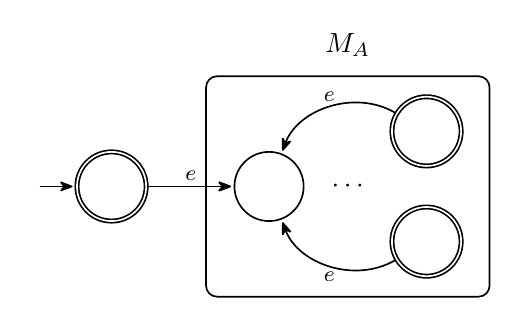
\begin{tikzpicture}[->,>={Stealth[round]},shorten >=1pt,%
        auto,node distance=2cm,on grid,semithick,
        inner sep=2pt,bend angle=50,initial text=]
        \node[initial,state,accepting]  at (-2, 0)  (q)     {};
        \node[initial,state]                        (q_0)   {};
        \node[state,accepting]          at (2,0.7)  (q_1)   {};
        \node[state,accepting]          at (2,-0.7) (q_2)   {};
        \node                           at (1,0)    (dots)  {$\cdots$};
        \node                           at (1,1.8)          {$M_A$};
        \draw[rounded corners] (-0.8,-1.4) rectangle (2.8,1.4);
        
        \path [every node/.style={font=\footnotesize}]
        (q)     edge                node         {$e$} (q_0)
        (q_1)   edge [bend right]   node [above] {$e$} (q_0)
        (q_2)   edge [bend left]    node [below] {$e$} (q_0);
    \end{tikzpicture}
\end{document}